%
%
\subsection{Die Natur des Lichts}
Es gibt zwei Vorstellungen zur Natur des Lichtes. Die eine ist die Wellentheorie, die andere
die korpuskulare Theorie. Diese Beiden scheinen auf den ersten Blick unvereinbar in der mathematischen
Beschreibung, welche einmal durch die Maxwellgleichungen (Wellentheorie) und ein anderes
mal durch die newtonsche Punktmechanik(korpuskulare Theorie) beschrieben werden. Es ist auch nur in der Quantenmechanik
möglich eine vollständig Beschreibung zu geben. Hier treten dann die beiden
Modelle als Grenzfälle auf.
Welches Modell nun zutrifft, hängt immer von dem Experiment ab.
So wird die Wellentheorie bei Beugung am Spalt oder Inteferenz benutzt und die Korpuskel beim lichtelektrichen
Effekt oder Comptoneffekt. Es l"asst sich also allgemein sagen, dass bei einer großen Anzahl an
Photonen, die man über die räumliche Ausbreitung mittelt, die Wellentheorie nimmt und
bei Wechselwirkungen mit Materie und Licht das Korpuskullmodell.

\subsection{Der Photoeffekt}
Es wird eine sich im Vakuum befindliche Festkörperoberfläche mit monochromatischem
Licht bestrahlt. Dieser Körper wird Photokathode genannt. Es wird der gegebenüber stehenden Elektrode
ein höheres Potential zugeteilt, damit die Elektronen von der Photokathode zu dieser gelenkt werden.
Es folgen die Ergebnisse:
 \begin{description}

\item[Die Zahl der pro Zeiteinheit ausgelösten Elektronen ist proportional zur Lichtintensität.]

\item[Eine Grenzfrequenz, unter welcher der Photoeffekt nicht mehr auftrit, existiert.]

\item[Die Energie der Photoelektronen (gemessen über ihre Geschwindigkeit) ist proportional zur Lichtfrequenz und unabhängig von der Lichtintensität.]

 \end{description}

Sämtliche Ergebnisse lassen sich nicht mit einem Wellenmodell erklären:
Wenn man beispielsweise annimmt, dass die Elektronen an der Oberfläche eines Metalles durch das elektrische Feld des einfallenden Lichtes zu erzwungenen Schwingungen angeregt werden, dann müssten die Elektronen die Metalloberfläche verlassen können, sobald ihre Schwingungsamplitude so groß geworden ist, dass sie die elektrostatischen, rück-treibenden Kräfte überwinden. Das heißt, dass auch bei langwelligem Licht mit ausreichend hoher Intensität der Photo-Effekt möglich sein müsste. Es müsste bei einer bestimmten Frequenz Resonanzphänomene zu beobachten sein, wo der Photo-Effekt bevorzugt auftritt. Weiterhin müsste die Energie der Photoelektronen mit der Lichtintensität anwachsen. All diese Forderungen stehen aber im Widerspruch zu den experimentellen Ergebnissen.

Mit dem korpuskel Modell kann man aber all diese Punkte erklären, denn ein Photon der Frequenz
$\nu$ hat eine Engergie von $h \nu$, wenn diese Energie gleich oder größer der Austrittsarbeit $A_k$ eines Elektron ist,
da das Photon diese übergibt, löst sich das Elektron aus dem Festkörper mit einer Geschwindigkeit, die aus $E_{kin}$ herrührt.
So kann man diese Gleichung aufstellen:
\begin{align}
h \nu = E_{kin} + A_k
\end{align}
Dies erklärt große Teile der Ergebnisse. Es ist nocht anzumerken, dass ein Photon nur ein Elektron lösen kann. Folglich sind die ausgelösten Elektronen proportional zur Lichtintensität.

\begin{figure}[h]
	\centering
		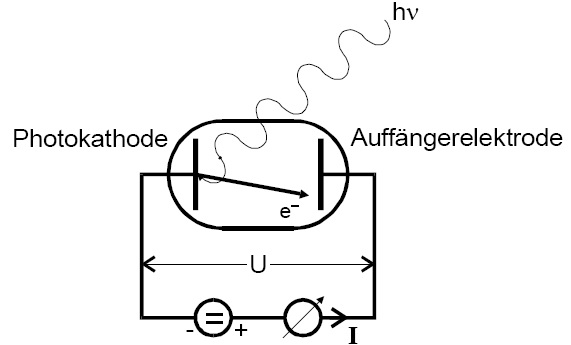
\includegraphics[width=1.00\textwidth]{PrinzipDesPhotoeffekts.jpg}
		\caption{Prinzip des Photoeffekts}
	\label{fig:PrinzipDesPhotoeffekts}
\end{figure}